\documentclass[letter]{article}
\usepackage[utf8]{inputenc}

\usepackage{tikz}
\usepackage{graphicx}
\usepackage{wrapfig}

\usepackage{mhsetup}
\usepackage{mathtools}

\usepackage{amssymb}
\usepackage{textcomp}
\usepackage{siunitx}

\usepackage[parfill]{parskip}
\usepackage{array}

\sisetup{separate-uncertainty,multi-part-units=single}
\numberwithin{equation}{section}
\graphicspath{ {./images/} }

\title{Experiment 7 — Standing waves in water}
\author{Laurence Amadeus Tristan, Nero Su, Weihong Deng}
\date{28/02/2019}

\begin{document}
\maketitle

\section{Purpose}
The purpose of this experiment is to figure out the speed of sound by examining the resonances of an open-ended resonance tube.

\section{Theory}
A standing wave consists two traveling waves interfering with each other in a particular manner that makes it appear stationary as a whole. As such, they consist of both nodes and antinodes. Nodes are positions where the particles in the air are stationary and not moving, whereas antinodes are the opposite of nodes, where the air particles moves back and forth at its greatest amplitude possible. One such example of a standing wave is resonance.

When resonance (i.e. standing waves) occurs, there will be a series of antinodes and nodes set in fixed locations along the air column.  This happens when the length of the air column \(L\) and the wavelength of the sound \(\lambda\) satisfies the equation:

\begin{equation} \label{eq:t1}
  L = N \ \frac{\lambda}{4}, \qquad N = \{1, 3, 5, \ldots\}
\end{equation}

\begin{tabbing}
  where \= \(L\) \= = length of air column, \\
  \> \(N\) \> = resonance order (odd integer values only, e.g. 1, 3, 5, \ldots), \\
  \> \(\lambda\) \> = wavelength of sound.
\end{tabbing}

Note that the length of the air column \(L\) does not equal to the length of the air chamber \(D\) in the tube, as the final antinode is located a distance \(x\) away from the open end of the tube. In terms of \(D\), this means that

\begin{equation} \label{eq:t2}
  L = D + x
\end{equation}

\begin{tabbing}
  where \= \(L\) \= = length of air column \\
  \> \(D\) \> = length of the air chamber, \\
  \> \(x\) \> = end correction.
\end{tabbing}

The end correction \(x\) is constant. This value depends on the diameter of the tube and the particular sound frequency that is made by the source, and cannot be dependent on the resonance order \(N\).

\section{Procedure}
\begin{wrapfigure}{r}{0.4\textwidth} 
  \centering
  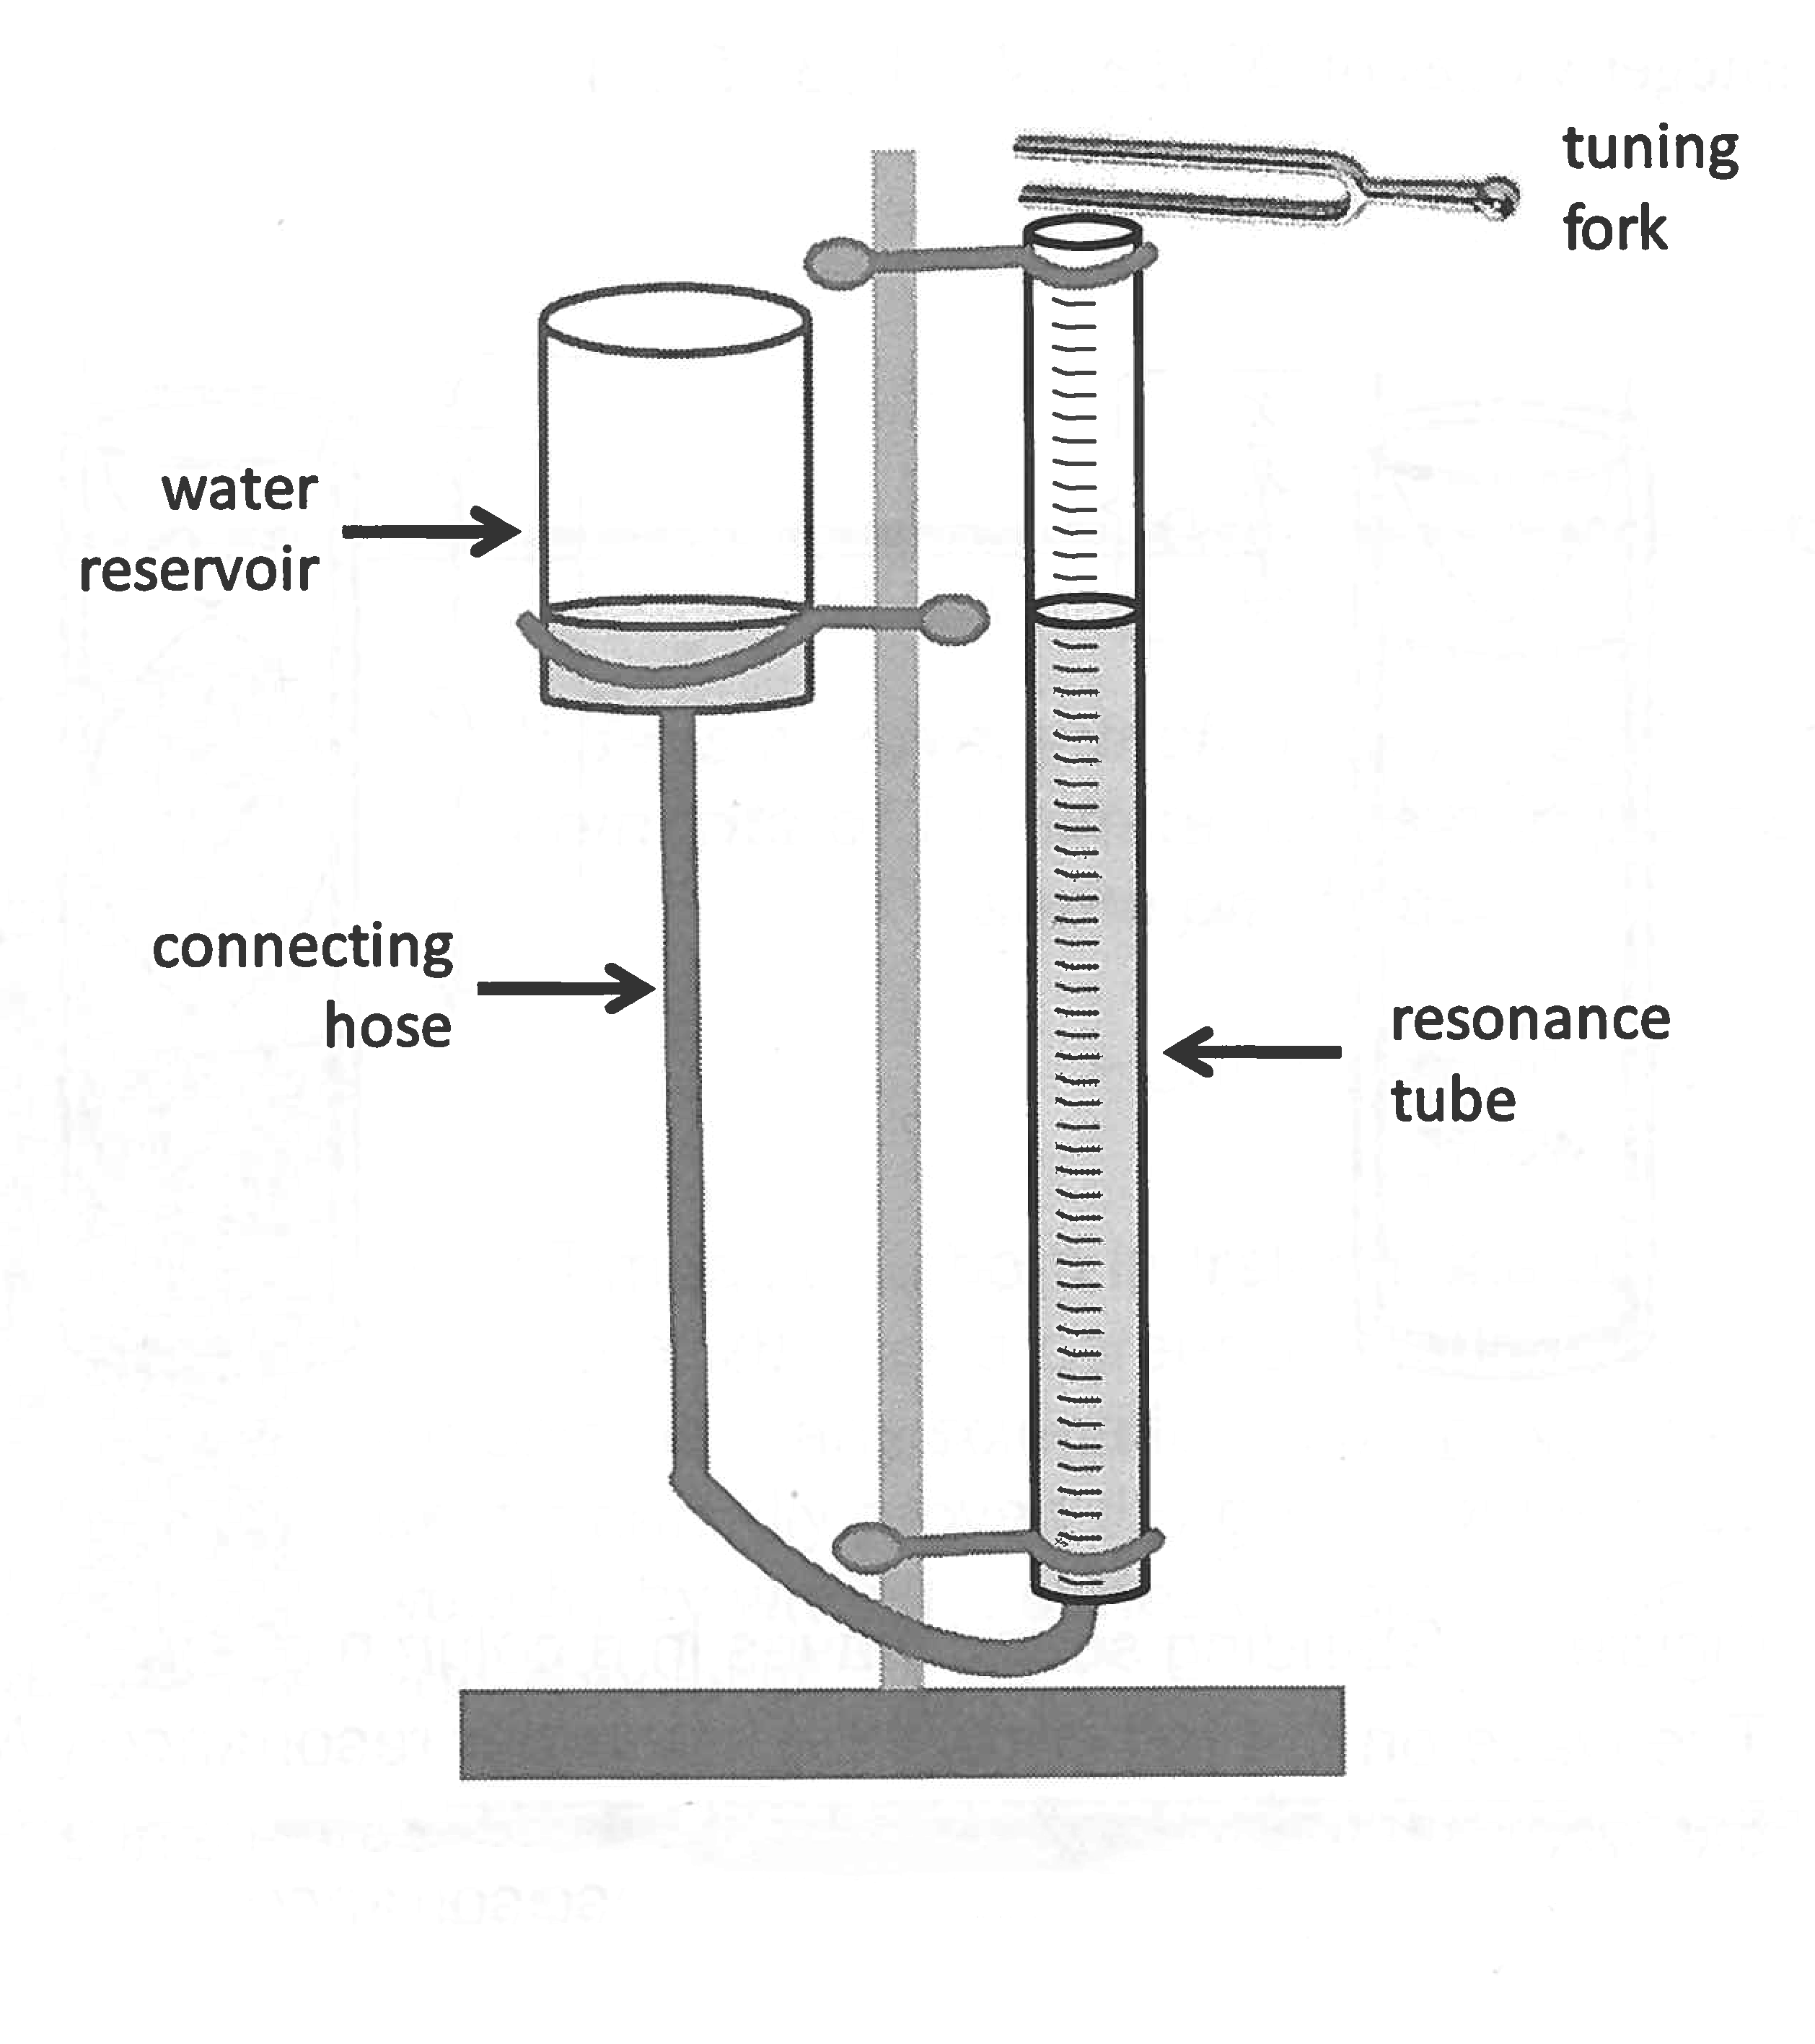
\includegraphics[width=0.4\textwidth]{drawing.png}
  \caption{Diagram of the apparatus}
  \label{fig:apparatus}
\end{wrapfigure}

Before starting the experiment, we first moved the apparatus to the floor of the laboratory. This was done to minimise the chance of breaking the apparatus due to human error. After that, we added a relatively small amount of water to the resevoir in order to increase the range of measurement.

First, we lower the water level in the tube as fast as possible by lowering the resevoir by hand (as in removed from the stand it was placed in). While doing so, gently strike a tuning fork with a rubber mallet and place it just above the resonance tube, taking great care to make sure that the fork do not make contact with the tube. This allows us to locate roughly the values of \(D\) of which resonance happens (in which it will give out a greatly amplified tone of the tuning fork).

Then, using our initial estimates for \(D\), we adjusted the water level so that it matches up with one of our estimates, and with a gently-struck tuning fork, we adjusted the water level continually until we found the value of \(D\) for which the tone experienced the most amplification. Repeat for the other estimates.

After that, we repeated the above procedures for every tuning fork that was provided. Those are listed at \ref{table:d1}. Note that for every \(D\) values that has resonance occuring, those value corresponds to the resonance order \(N\), which has been defined in Equation \eqref{eq:t1}. For most of the tuning forks available to us, only \(N = 1\) and \(N = 3\) resonances were observed, and \(N = 5\) was only observed for the tuning fork with the highest frequency.

\pagebreak
\section{Data}
\begin{table}[!h]
  \centering
  \begin{tabular}{|c|l|l|}
    \hline
    Experiment no.  & Note value            & Frequency (\(f\))/\si{Hz} \\
    \hline
    1               & \(\mathrm{F}_4\)      & 349.2 \\
    2               & \(\sim \mathrm{G}_4\) & 392 \\
    3               & \(\sim \mathrm{A}_4\) & 486.7 \\
    4               & \(\mathrm{C}_5\)      & 523.2 \\
    \hline
  \end{tabular}
  \caption{Description of each experiment}
  \label{table:d1}
\end{table}

\begin{table}[!h]
  \centering
  \begin{tabular}{|l|l|l|}
    \hline
    Variable  & Value                       & Description\\
    \hline
    \(T_C\)   & \SI{24(1)}{\celsius}        & {Room temperature in Celsius}\\
    \(d\)     & \SI{3.366(2)}{\centi\metre} & {Inner diameter of the resonance tube}\\
    \(v_0\)   & \SI{331}{\metre\per\second} & {Speed of sound in air at \SI{0}{\celsius} (\SI{273}{\kelvin})}\\
    \hline
  \end{tabular}
  \caption{List of measured constant variables in the experiment}
  \label{table:d2}
\end{table}

\begin{table}[!h]
  \centering
  \begin{tabular}{|l|l|l|l|l|}
    \hline
    \(N\) & \(D_1 / \pm 1\) \si{cm} & \(D_2 / \pm 1\) \si{cm} & \(D_3 / \pm 1\) \si{cm} & \(D_4 / \pm 1\) \si{cm} \\
    \hline
    1  & 24  & 21  & 19  & 15 \\
    3  & 73  & 65  & 59  & 48 \\
    5  & --  & --  & --  & 81 \\
    \hline
  \end{tabular}
  \caption{Experimental data for all four experiments}
  \label{table:d3}
\end{table}

\section{Analysis}
Combine equations \eqref{eq:t1} and \eqref{eq:t2} and solve for \(D\).
\begin{align} \label{eq:a1}
  \frac{N \lambda}{4} &= D + x \notag \\
  -D &= - \left (\frac{N \lambda}{4} \right) + x \notag \\
  D &= N \left(\frac{\lambda}{4} \right) - x
\end{align}

As the wavelength \(\lambda\) is constant for each tuning fork, we can safely assume that Equation \eqref{eq:a1} is linear. As such, \(\frac{\lambda}{4}\) is the gradient of the linear function, and the error correction \(x\) is the \textit{y}-intercept of the function. As such, for brevity we do the following substitution:

\begin{equation}
  m = \frac{\lambda}{4}
\end{equation}  

With the data from \ref{table:d3} (and after converting the measurements to metres) and Equation \eqref{eq:a1}, we were able to draw Figure \ref{fig:plot1} of \(D_4\) as a function of \(N\).

\pagebreak

\begin{figure}[!h]
  \centering
  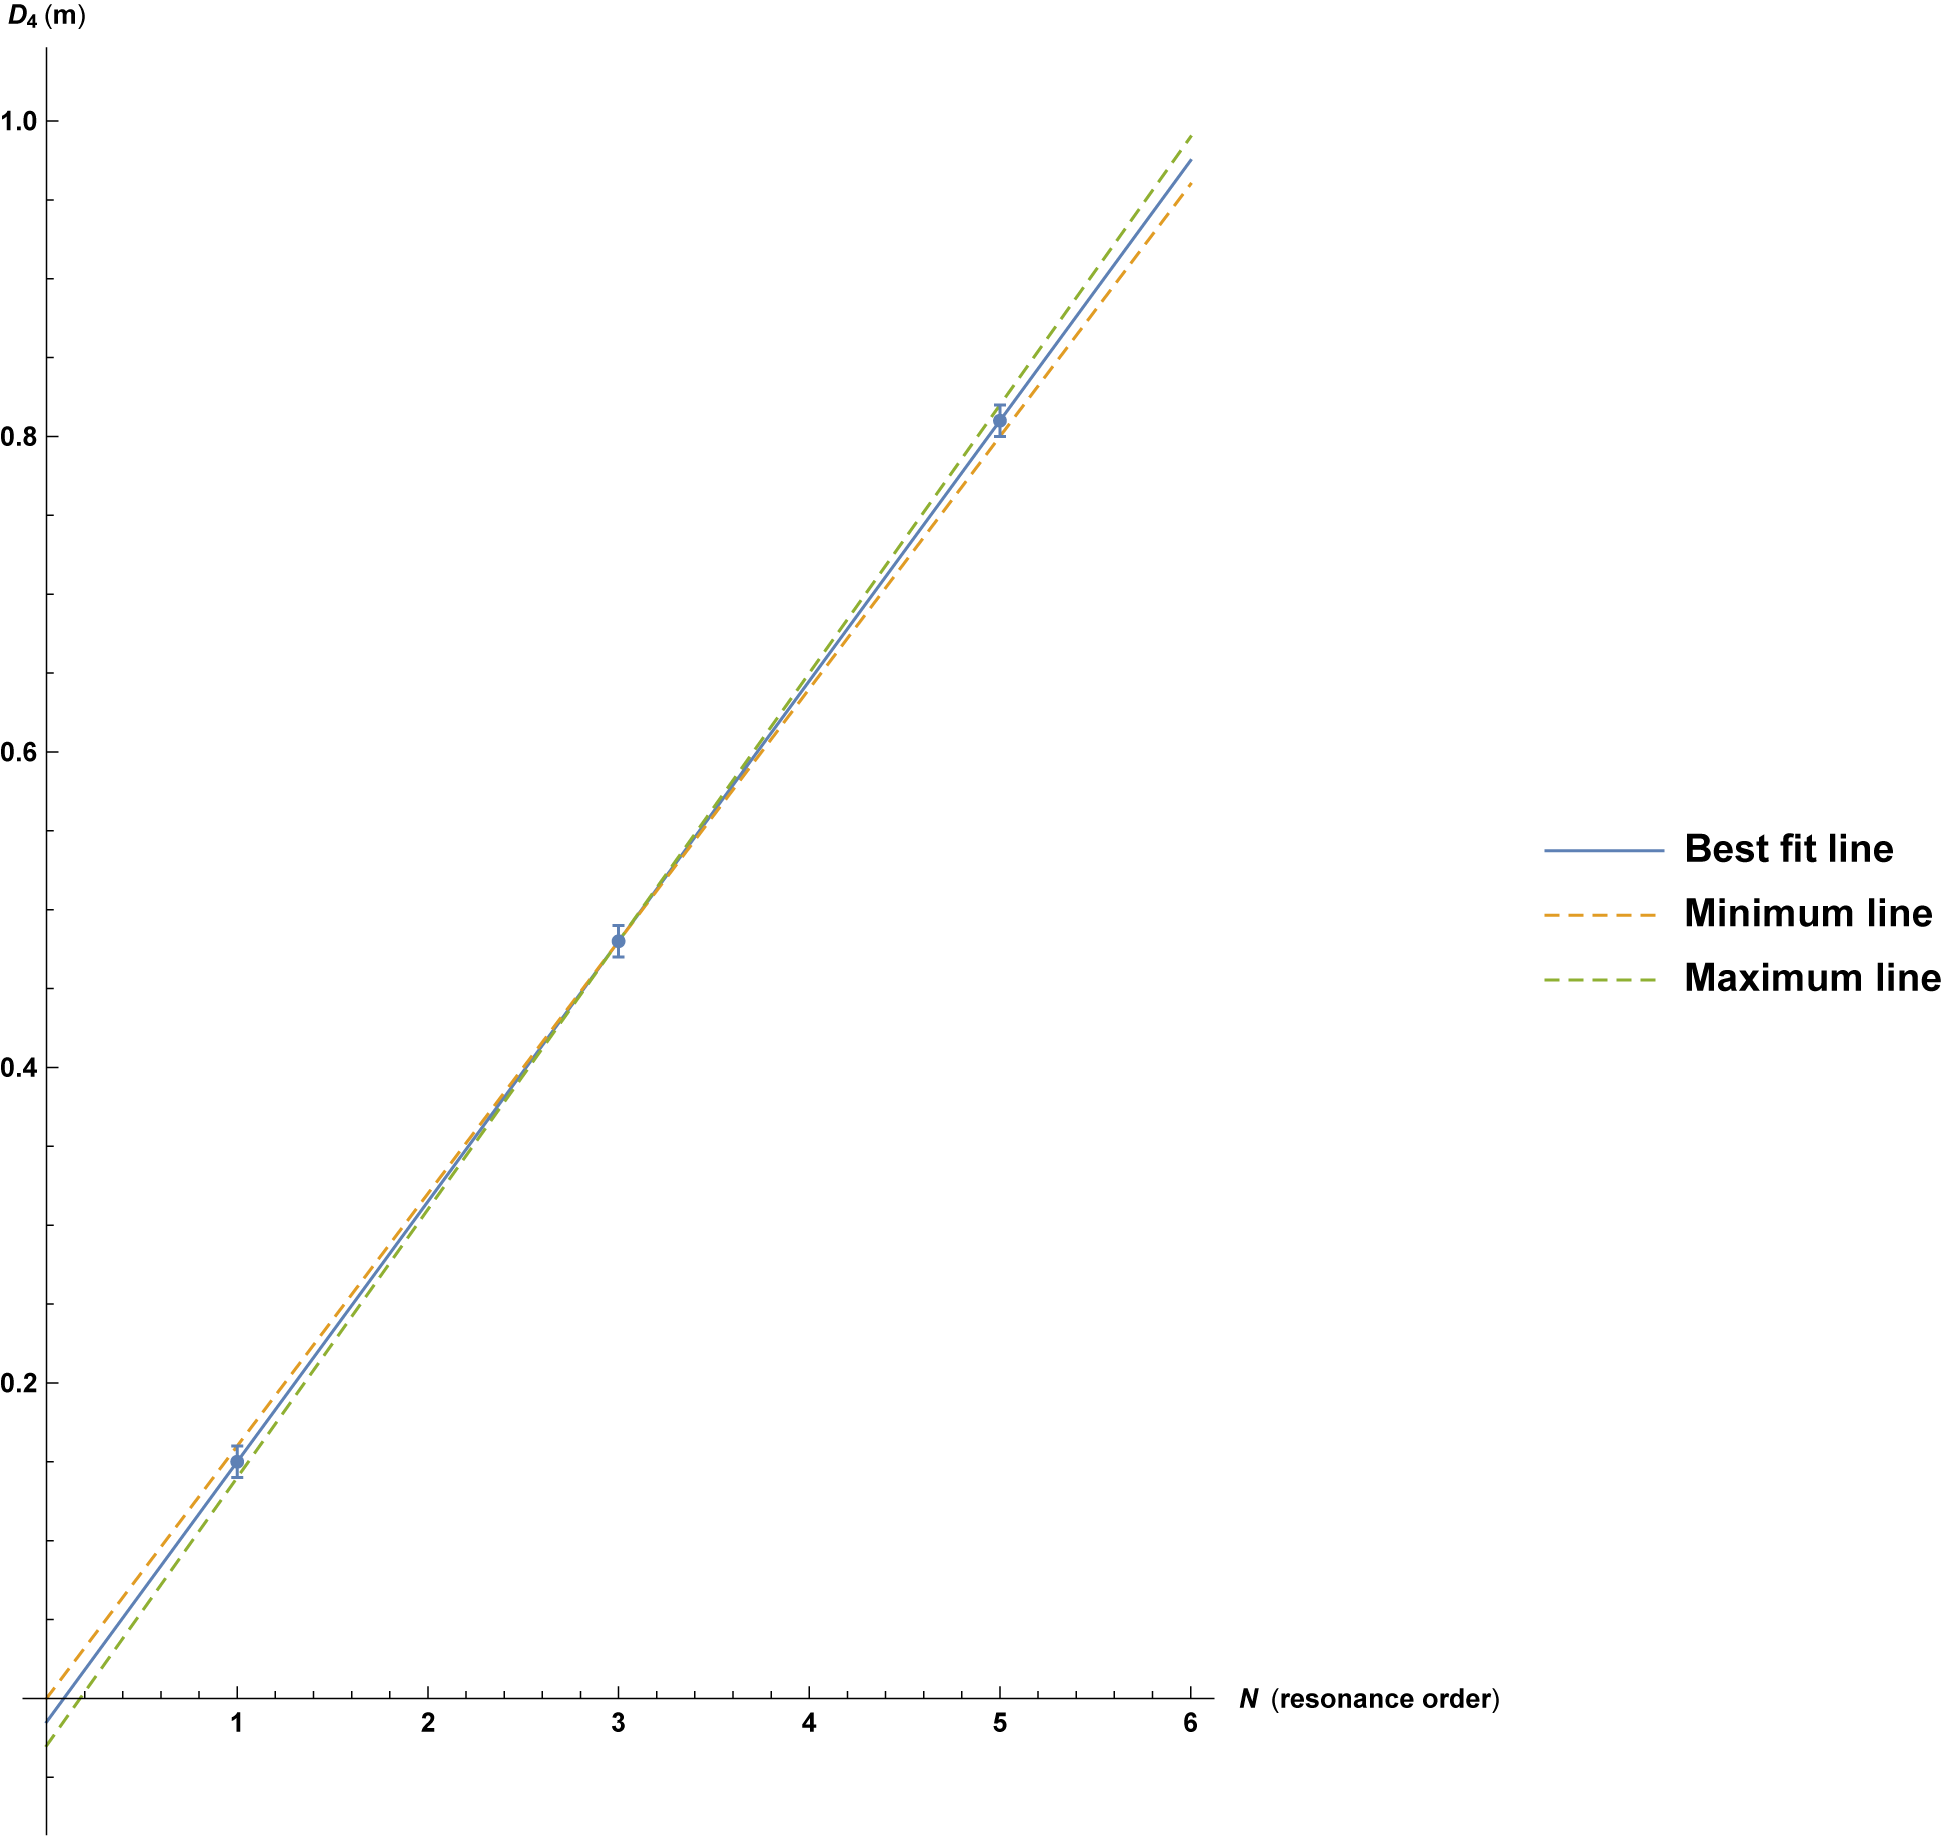
\includegraphics[width=0.75\textwidth]{plot_pdf.png}
  \caption{Plot of the length of air column \(D_4\) against the resonance order \(N\).}
  \label{fig:plot1}
\end{figure}

Now, get the value of both \(m\) and \(x\) for Figure \ref{fig:plot1}, and calculate its uncertainties.

\begin{align*}
  m &= \frac{\SI{0.81}{m} - \SI{0.15}{m}}{5 - 1} \\
  &= \SI{0.165}{m}
\end{align*}
\begin{align*}
  \delta m &= m_{\mathrm{best}} - m_{\mathrm{min}} \\
  &= \frac{\SI{0.81}{m} - \SI{0.15}{m}}{5 - 1} - \frac{\SI{0.80}{m} - \SI{0.14}{m}}{5 - 1} \\
  &= \SI{0.165}{m} - \SI{0.16}{m} \\
  &= \SI{0.005}{m}
\end{align*}
\begin{equation*}
  \therefore m = \SI{0.165(5)}{m}
\end{equation*}

By observation,
\begin{align*}
  x &= \SI{-0.015}{m}, \\
  x_\mathrm{min} &= \SI{0}{m}
\end{align*}
\begin{align*}
  \delta x &= |x_{\mathrm{best}} - x_{\mathrm{min}}| \\
  &= |\SI{-0.015}{m} - \SI{0}{m}| \\
  &\approx \SI{0.02}{m}
\end{align*}
\begin{equation*}
  \therefore x = \SI{-0.02(2)}{m}
\end{equation*}

For the rest of the experimental data (Experiment 1 to 3), we assume that the best-fit line goes through the two data points. The uncertainties for the values of \(\lambda\) and \(x\) can be assumed to be similar, if not identical, for all forks. Because of that, the calculations needed to determine \(m\) and \(x\) quite similar to the calculations done for Experiment 4. The following is an example calculation for Experiment 1:


\section{Discussion}


\end{document}
